\hypertarget{chap:related}{\chapter{Related Works}}
\label{chap:related-work}
\section{Datasets}\label{sec:dataset}
\subsection{Stanford Sentiment Treebank} \label{sec:sst}
In this thesis, we used Standford Sentiment Treebank (SST) dataset~\cite{socher2013recursive} to evaluate our models sentence-level sentiment analysis task.
Originally, the dataset was built based on Rotten Tomatoes Movie Review dataset~\cite{Rotten-Tomato}~\cite{socher2013recursive}.
In total, Standford Sentiment Treebank contains 11,855 sentences.
The dataset was split into training, validation and testing set which contains 8544, 1101 and 2210 sentences respectively (Fig.\ref{fig:sstfinegrain}).
Table \ref{table:sststatistic} shows the distribution of sentiment classes on training, validation and testing set.

In this dataset, every sentence was parsed using Stanford (constituency) parser~\cite{socher2013recursive}\footnote{Open source tool: \url{https://stanfordnlp.github.io/CoreNLP/}}, each phrase which is spanned by any sub-tree of the parse tree is then labeled with  a fine-grained sentiment label (see \textbf{Figure \ref{fig:sst}}).
Fine-grained sentiment is a setting which partition all sentiments into 5 classes: "Positive", "Somewhat Positive", "Neutral", "Somewhat Negative" and "Negative"~\cite{socher2013recursive} (a.k.a. \textbf{Fine-grained setting}).
There are total 215,154 phrases in the whole dataset.

For \textbf{Binary setting}, there are only to sentiment classed on the entire dataset, which means all neutral sentiment sentences are removed, "Positive" and "Somewhat Positive" are merged into one class, the same rule applied on "Somewhat Negative" and "Negative"~\cite{socher2013recursive}.
After all "Neutral" sentences have been removed, there are 6920/872/1821 sentences remained in train/dev/test set (Fig. \ref{fig:sstbinary}).


Table \ref{table:sststatistic} show statistics by sentences of Sentiment Treebank Dataset.
SST dataset is publicly available online\footnote{https://nlp.stanford.edu/sentiment/index.html}.

\begin{figure}[H]
    \begin{minipage}{\textwidth}
        \centering
        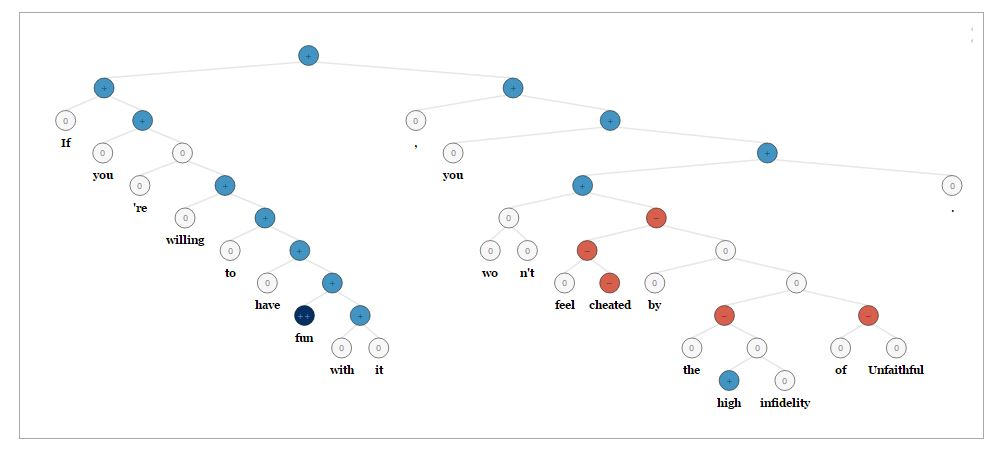
\includegraphics[width=0.9\linewidth]{figure/sst}
        \caption[A parsed sentence in SST]{A parsed sentence in SST\footnote{Render by Pytreebank \url{https://github.com/JonathanRaiman/pytreebank}}}
        \label{fig:sst}
    \end{minipage}
\end{figure}

\begin{figure}[H]
    \begin{minipage}{\textwidth}
        \centering
        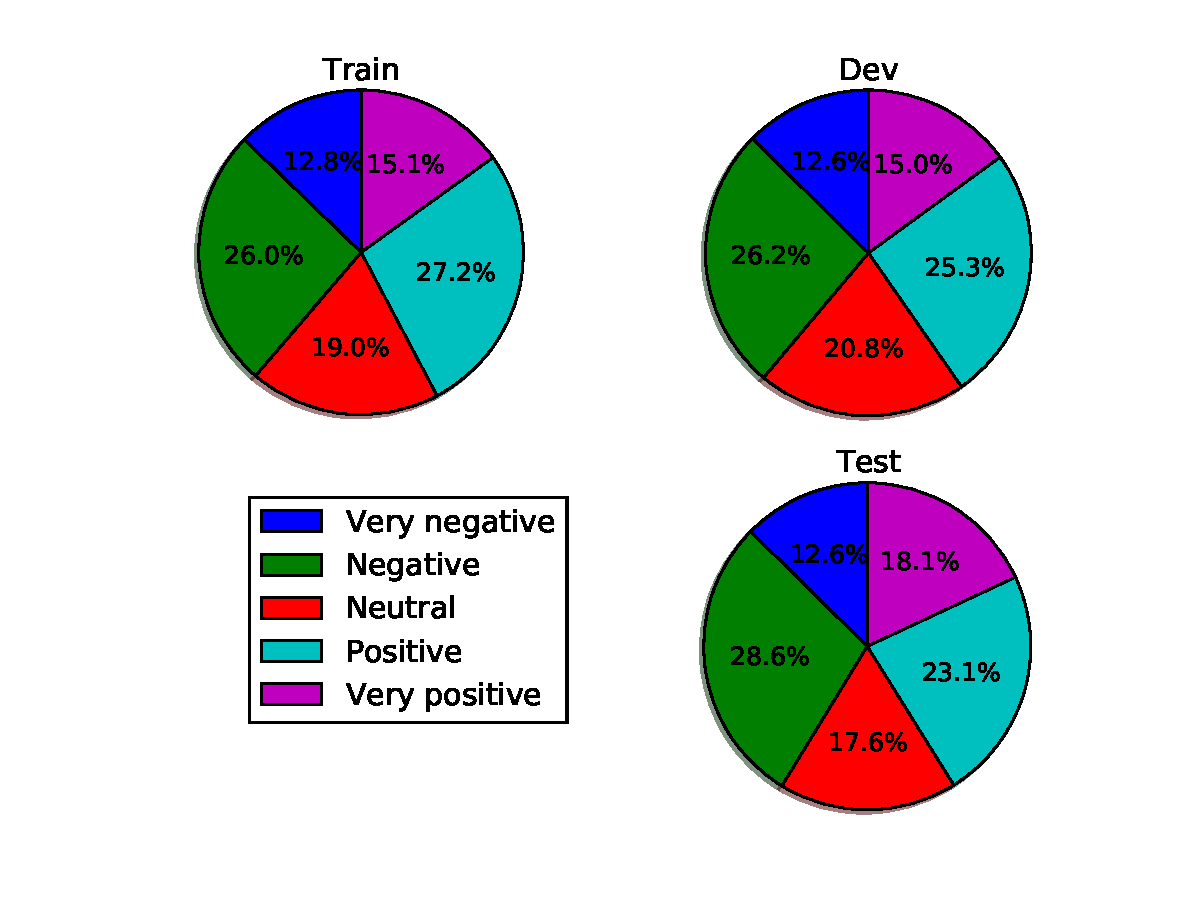
\includegraphics[width=0.9\linewidth]{figure/sstfinegrain}
        \caption[SST fine-grain sentiment distribution]{SST fine-grain sentiment distribution}
        \label{fig:sstfinegrain}
    \end{minipage}
\end{figure}

\begin{figure}[H]
    \begin{minipage}{\textwidth}
        \centering
        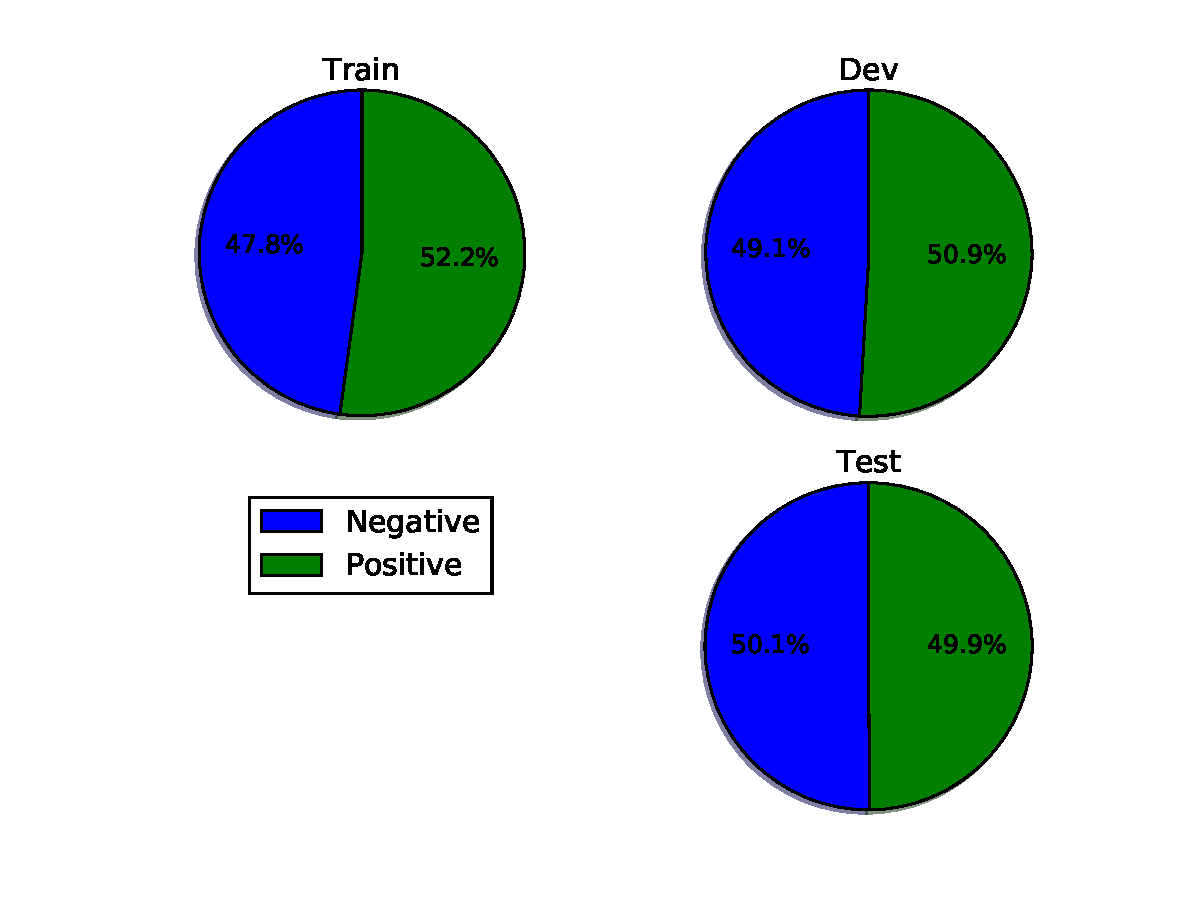
\includegraphics[width=0.9\linewidth]{figure/sstbinary}
        \caption[SST binary sentiment distribution]{SST binary sentiment distribution}
        \label{fig:sstbinary}
    \end{minipage}
\end{figure}

% Please add the following required packages to your document preamble:
% \usepackage{multirow}
\begin{table}[H]
    \centering
    \caption{SST statistics}
    \label{table:sststatistic}
    \begin{tabular}{lllll}
        Number of review       &               &      &                       &  \\ \cline{1-4}
        \multirow{5}{*}{Train} & Very Negative & 1092 & \multirow{2}{*}{3310} &  \\ \cline{2-3}
        & Negative      & 2218 &                       &  \\ \cline{2-4}
        & Neutral       & 1624 &                       &  \\ \cline{2-4}
        & Positive      & 2322 & \multirow{2}{*}{3610} &  \\ \cline{2-3}
        & Very positive & 1288 &                       &  \\ \cline{1-4}
        \multirow{5}{*}{Dev}   & Very Negative & 139  & \multirow{2}{*}{428}  &  \\ \cline{2-3}
        & Negative      & 289  &                       &  \\ \cline{2-4}
        & Neutral       & 229  &                       &  \\ \cline{2-4}
        & Positive      & 279  & \multirow{2}{*}{444}  &  \\ \cline{2-3}
        & Very positive & 165  &                       &  \\ \cline{1-4}
        \multirow{5}{*}{Test}  & Very Negative & 279  & \multirow{2}{*}{912}  &  \\ \cline{2-3}
        & Negative      & 633  &                       &  \\ \cline{2-4}
        & Neutral       & 389  &                       &  \\ \cline{2-4}
        & Positive      & 510  & \multirow{2}{*}{909}  &  \\ \cline{2-3}
        & Very Positive & 399  &                       &  \\ \cline{2-4}
    \end{tabular}
\end{table}

\subsection{Amazon Reviews dataset}\label{sec:amazon}
Amazon Reviews is a gigantic review dataset
which contains 142.8 million reviews from Amazon spanning May 1996 - July 2014\footnote{\url{http://jmcauley.ucsd.edu/data/amazon/}}.
Each review contains product review (rating, text, helpfulness vote) and metadata (descriptions, category information, price, brand, and image features)~\cite{amazon-reviews}.
In this thesis, we only used a small part of Amazon Reviews.
These parts include Amazon Movies and TV reviews (7,850,072 reviews)~\cite{mcauley2013hidden}, Amazon Book reviews (22,507,155 reviews) and the new Movies and TV reviews (4,607,047 reviews)~\cite{McAuleyTSH15}~\cite{HeM16}.

Listing \ref{lst:amzreview} is a sample of book reviews.
Amazon Book reviews and new Movies and TV dataset have the same format. Listing \ref{lst:oldamzreview} is a sample of Amazon Movies and TV reviews old dataset (7,850,072 reviews).

\begin{lstlisting}[caption={Amazon reviews sample},label={lst:amzreview}]
    {
        "reviewerID": "AH2L9G3DQHHAJ",
        "asin": "0000000116",
        "reviewerName": "chris",
        "helpful": [5, 5],
        "reviewText": "Interesting Grisham tale of a lawyer that takes millions of dollars from his firm after faking his own death. Grisham usually is able to hook his readers early and ,in this case, doesn't play his hand to soon. The usually reliable Frank Mueller makes this story even an even better bet on Audiobook.",
        "overall": 4.0,
        "summary": "Show me the money!",
        "unixReviewTime": 1019865600,
        "reviewTime": "04 27, 2002"
    }
\end{lstlisting}

\begin{lstlisting}[caption={Old Amazon reviews sample},label={lst:oldamzreview}]
{
"reviewerID": "AH2L9G3DQHHAJ",
"asin": "0000000116",
"reviewerName": "chris",
"helpful": [5, 5],
"reviewText": "Interesting Grisham tale of a lawyer that takes millions of dollars from his firm after faking his own death. Grisham usually is able to hook his readers early and ,in this case, doesn't play his hand to soon. The usually reliable Frank Mueller makes this story even an even better bet on Audiobook.",
"overall": 4.0,
"summary": "Show me the money!",
"unixReviewTime": 1019865600,
"reviewTime": "04 27, 2002"
}
\end{lstlisting}

The differences between the old Amazon reviews dataset\footnote{\url{https://snap.stanford.edu/data/web-Amazon.html}} and new Amazon reviews dataset\footnote{\url{http://jmcauley.ucsd.edu/data/amazon/}} is that:
They were gathered using different crawling methods, the author also solved the duplication problem in new the dataset~\cite{amazon-reviews}.
Table \ref{table:moviereview} shows number of reviews by overall.

\begin{table}[H]
    \centering
    \caption{New Movies and TV dataset}
    \label{table:moviereview}
    \begin{tabular}{@{}lllc@{}}
        \toprule
        & \multicolumn{3}{l}{Number of reviews}                         \\ \midrule
        5-Star & 2761408 & \multirow{2}{*}{3618913} & \multirow{5}{*}{4607047} \\ \cmidrule(r){1-2}
        4-Star & 857505  &                          &                          \\ \cmidrule(r){1-3}
        3-Star & \multicolumn{2}{l}{415369}         &                          \\ \cmidrule(r){1-3}
        2-Star & 233221  & \multirow{2}{*}{572765}  &                          \\ \cmidrule(r){1-2}
        1-Star & 339544  &                          &                          \\ \bottomrule
    \end{tabular}
\end{table}


\section{Neural network architects for sentence composition}\label{sec:composer}
\subsection{Recurrent neural networks (RNNs)}\label{sec:RNN}
In real life, we usually encounter a type of problems whose output (or output sequence) is determined by a variable-length sequence of input data points.
Recurrent Neural Networks have been proven to be effective network architects when applying on this type of problems.
Particularly in Natural Language Processing, various tasks enjoy dramatic improvements by using different variations of Recurrent Neural Networks, these tasks include:  speech recognition~\cite{speech-lstm}~\cite{MiaoGM15}, sentiment analysis~\cite{treeLSTM}~\cite{cnn-rnn}~\cite{attention-gru}, text summarization~\cite{RushCW15}~\cite{NallapatiXZ16}, machine translation~\cite{FiratCB16}~\cite{SutskeverVL14}~\cite{BritzGLL17}, language modeling~\cite{mikolov-nlm}~\cite{JozefowiczVSSW16} and more~\cite{deep-nlp}~\cite{Schmidhuber14}~\cite{deeplearning-book}.

By definition, Recurrent Neural Networks are any Neural Networks which have at least a recurrent connection~\cite{rnn-def} but we will describe several common types of Recurrent Neural Networks which closely related to this theses.

\subsubsection{Vanilla Recurrent Unit}\label{sec:vanilla-rnn}
Denoting input sequence as \(I = \{i_0,\ldots,i_n\}, \forall t, i_t \in \mathbb{R}^n\), Vanilla Recurrent unit can be expressed as the following recursive formula~\cite{treeLSTM}:
\begin{align}
      h_t &= tanh(Wi_t + Uh_{t-1} + b)&\label{eq:rnn}
\end{align}
In Eq.\ref{eq:rnn}, \(h_t\) is called state of the system~\cite{deeplearning-book}, but we can also treat \(h_t\) as an output of the unit.
In that sense, the system output sequence would be \(O = \{h_0,\ldots,h_n\}, \forall t, h_t \in \mathbb{R}^m\) but in some problems/settings (e.g. \hyperref[sec:sent-level]{sentence-level sentiment analysis}, machine translation~\cite{SutskeverVL14}), we only use the last output \(h_n\).
The output (output sequence) can be treated as input for other neural networks (e.g. MLP, CNN or even RNN).

For demonstration, the computing process of the network can be unfolded as in Fig.\ref{fig:rnn-unfold}.
The network is trained using back propagation through it computational graph in Fig.\ref{fig:rnn-unfold}, which is called Back Propagation Through Time (BPTT)~\cite{BPTT}.
The number of time steps \(t\) to back propagate can be limited; this modification is named truncated BPTT~\cite{truncatedBPTT}.
Not only Vanilla RNN, but other recurrent architects can also be trained using BPTT.

\begin{figure}[H]
    \centering
    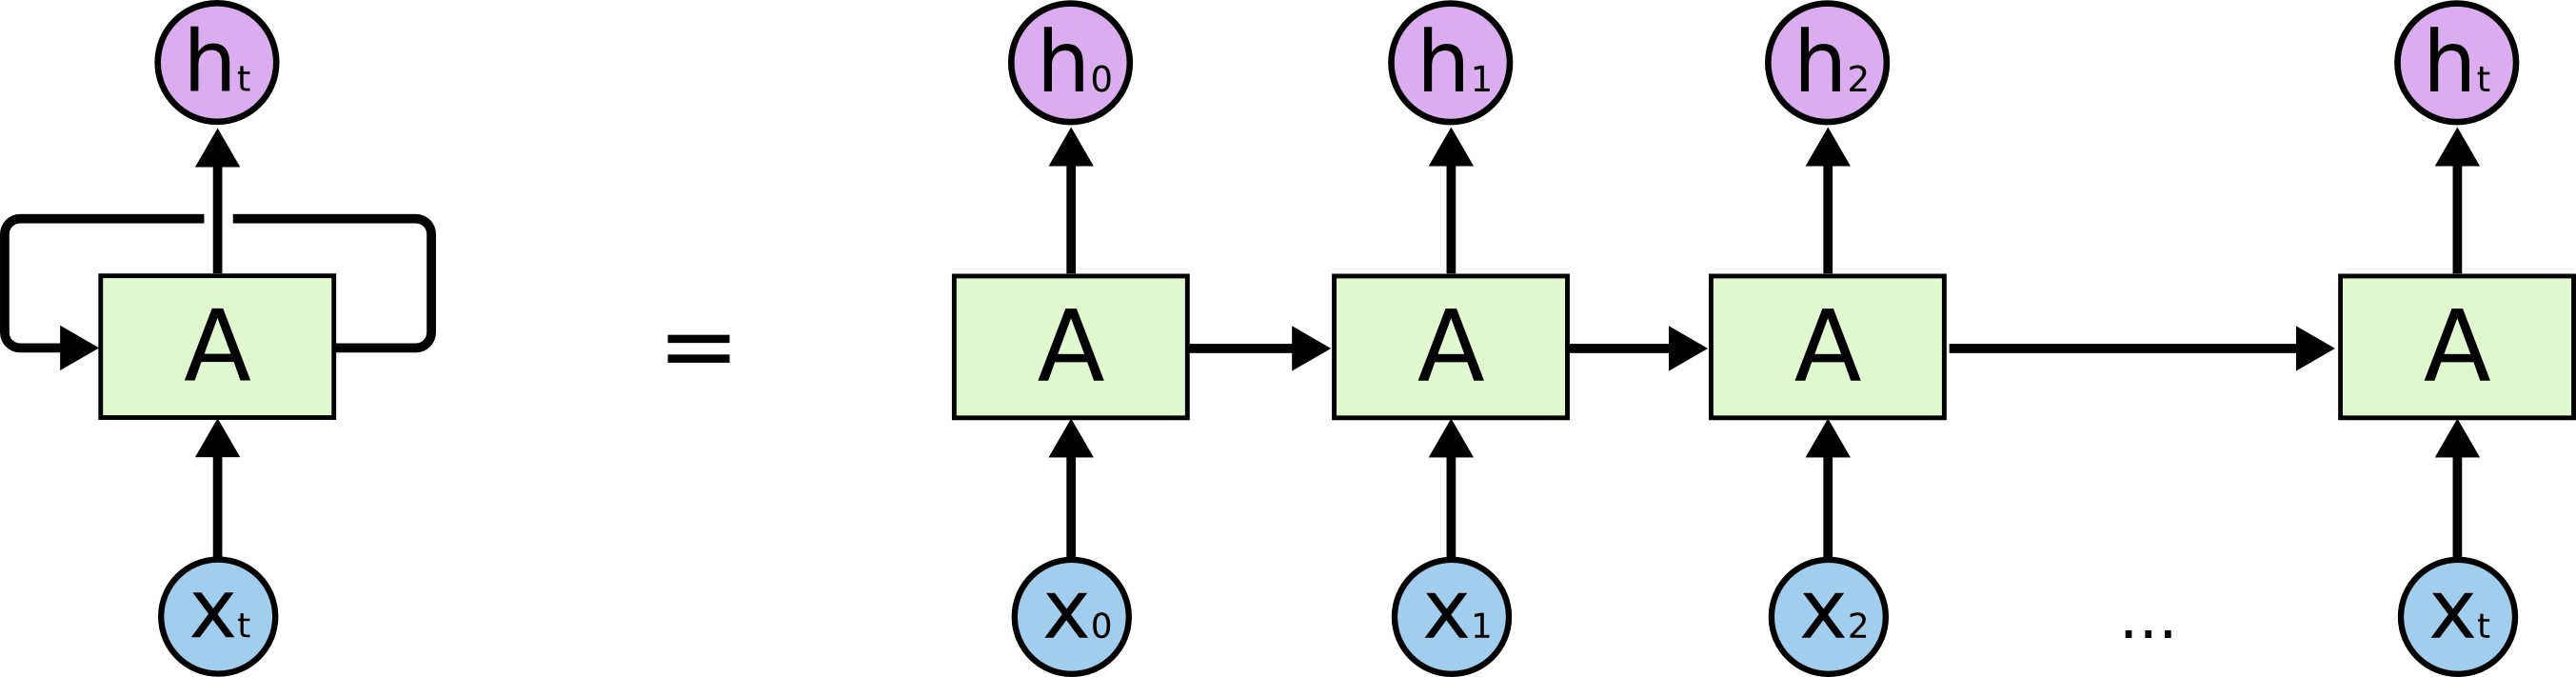
\includegraphics[scale=0.4]{figure/rnn-unroll}
    \caption[Vanilla Recurrent Neural Network]{Computational graph of Vanilla Recurrent Neural Network on an input sequence~\cite{colah-lsmt}.}
    \label{fig:rnn-unfold}
\end{figure}
\label{sec:gradient-vanish}
In theory, Vanilla Recurrent Neural Network is Turing-Complete~\cite{rnn-turing-complete} but  hard to train (especially on long input sequence) due to the problems of exploding and vanishing gradient~\cite{Bengio1994}.
To scratch the surface, given an output \(h_{t1}\) and a trainable parameter \(W\) at time \(t_2\) which denoted as \(W^{(t_2)}\),  exploding (vanishing) gradient can be understood as the norm \(L2\) of the gradient \(\frac{\partial h_{t1}}{\partial W^{(t_2)}}\) get exponentially bigger (smaller) with respect to the number of time steps \((t_1-t_2)\)~\cite{Bengio1994}.
In layman's terms, the longer the dependencies between an output and an input the (exponentially ) harder it is for the training process to capture those dependencies.
This phenomenon is demonstrated in Fig.\ref{fig:gradient-vanish}.

\begin{figure}[H]
    \centering
    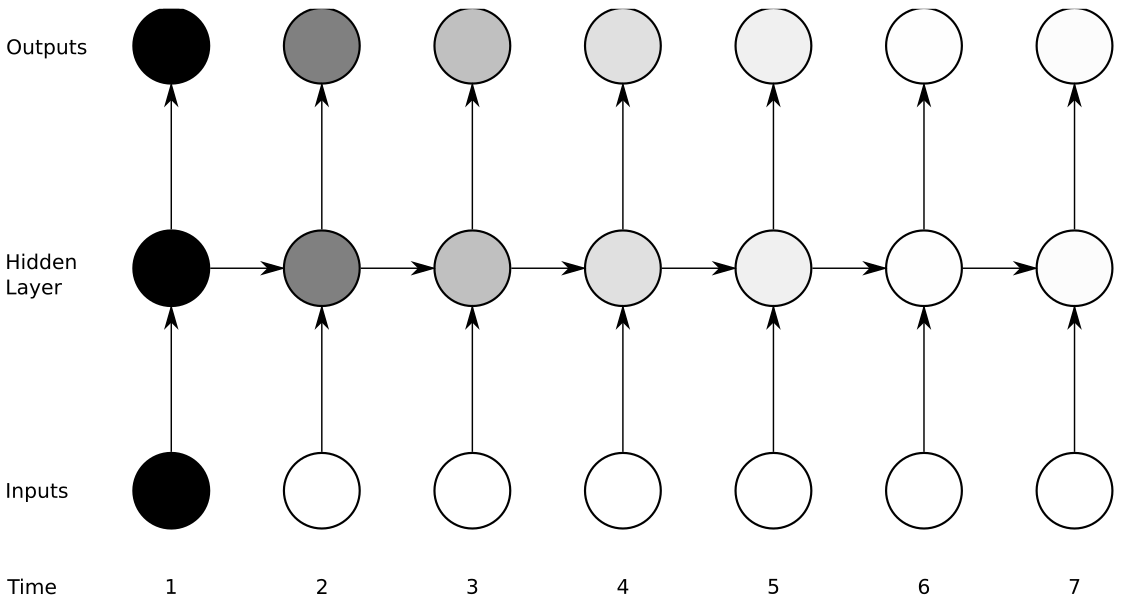
\includegraphics[scale=0.37]{figure/gradient-vanish}
    \caption[Gradient exploding (vanishing) on RNN]{Our main focus is on the first input.
    The shadings on the nodes indicate how much those nodes are affected when the value of the first input changed.
    More technically, denoting the first input as \(i_1\), the shading's intensity of a node \(n\) is calculated as \(\norm{\frac{\partial n}{\partial i_1}}\).
    The shading's intensity of nodes decrease exponentially through time steps.~\cite{Graves-thesis}}
    \label{fig:gradient-vanish}
\end{figure}

For exploding gradient, an ad-hoc technique called gradient clipping~\cite{hardRNN} was introduced and proven to be effective when being applied to many types of RNNs.
Given a gradient \(G\) that we are going to use to update our parameters, if it norm \(L2\) exceeds a threshold \(m\) we will clip it by this formula:
\begin{align}
      G &:= \frac{Gm}{\norm{G}} &
\end{align}
To mitigate the problem of vanishing gradient, Long Short Term Memory unit (LSTM)~\cite{originLSTM} unit was invented.


\subsubsection{Long Short Term Memory Unit}\label{sec:lstm}
Given a input sequence \(I = (i_0,\ldots,i_n), \forall t, i_t \in \mathbb{R}^n\), Long Short Term Memory unit can be expressed as the following recursive formula~\cite{treeLSTM}:
\begin{align}
    w_t &= \sigma(W^{(w)}i_t + U^{(w)}h_{t-1} + b^{(w)}) \label{eq:lstm-input-gate}&\\
      f_t &= \sigma(W^{(f)}i_t + U^{(f)}h_{t-1} + b^{(f)}) \label{eq:lstm-forget-gate}&\\
      o_t &= \sigma(W^{(o)}i_t + U^{(o)}h_{t-1} + b^{(o)}) \label{eq:lstm-output-gate}&\\
      u_t &= tanh(W^{(u)}i_t + U^{(u)}h_{t-1} + b^{(u)}) \label{eq:lstm-update-gate}&\\
      c_t &= r_t \otimes u_t + f_t \otimes c_{t-1} \label{eq:longterm-mem}&\\
      h_t &= o_t \otimes tanh(c_t) \label{eq:temperal-mem}&
\end{align}
In the formula above, operator \(\otimes\) is the Hadamard product~\cite{element-prod}.
The role of \(h_t\) in LSTM unit is similar to its role in \hyperref[sec:vanilla-rnn]{Vanilla Recurrent unit}.
Traditionally, \(w_t\), \(f_t\) and \(o_t\) are called input/write gate, forget/deallocate gate and output/read gate respectively.
In addition, \(c_t\) is called memory cell.
The output sequence of the LSTM unit is analogous to that of a Vanilla Recurrent unit output sequence \(O = \{h_0,\ldots,h_n\}\).

Intuitively, we can interpret how the network works as follow: in the above formula, \(h_{t-1}\) can be viewed as a short-term memory of the network; \(u_t\) is the information extracted from in current input \(i_t\) and the short-term memory \(h_{t-1}\); write gate \(w_t\) decides which information from \(u_t\) will be written into the memory cell \(c_t\); forgot gate \(f_t\) decides which information while be preserved on memory cell \(c_t\); and \(o_t\) decides which information will be read from the memory cell \(c_t\), which will produce the short-term memory (or output) \(h_t\).
A LSTM illustrated in Fig.\ref{fig:lstm}.

\begin{figure}[H]
    \centering
    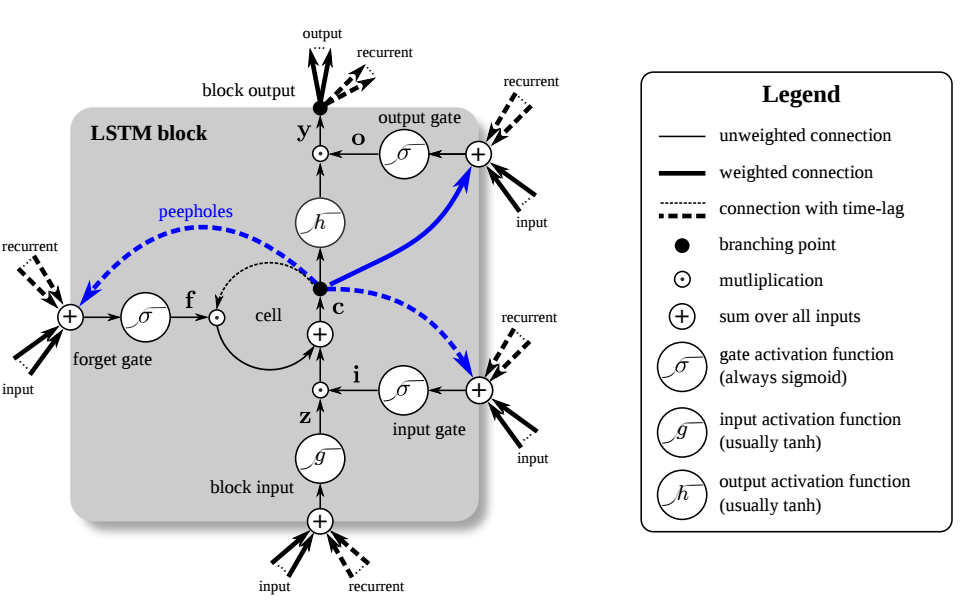
\includegraphics[scale=0.4]{figure/lstm}
    \caption[LSTM unit]{Diagram of a LSTM unit (excluded blue connections). Blue connections are added in a peephole LSTM.~\cite{lstm-search}}
    \label{fig:lstm}
\end{figure}


Other variations on LSTM include adding peephole to three gates of LSTM~\cite{peephole} which resulting in the following modification~\cite{colah-lsmt}:
\begin{align}
    w_t &= \sigma(W^{(w)}i_t + U^{(w)}h_{t-1} + \bm{V^{(w)}c_{t-1}} + b^{(w)}) &\\
      f_t &= \sigma(W^{(f)}i_t + U^{(f)}h_{t-1} + \bm{V^{(f)}c_{t-1}} + b^{(f)}) &\\
      o_t &= \sigma(W^{(o)}i_t + U^{(o)}h_{t-1} + \bm{V^{(o)}c_{t-1}} + b^{(o)}) &\\
      u_t &= tanh(W^{(u)}i_t + U^{(u)}h_{t-1} + b^{(u)}) &\\
      c_t &= r_t \otimes u_t + f_t \otimes c_{t-1} &\\
      h_t &= o_t \otimes tanh(c_t) &
\end{align}

\label{sec:GRU}
Another variation of LSTM unit is GRU unit~\cite{GRU}.
The formula of a  GRU unit can be expressed as follow~\cite{colah-lsmt}:
\begin{align}
    z_t &= \sigma(W^{(z)}i_t + U^{(z)}h_{t-1} + b^{(z)}) \label{eq:gru-update}&\\
      r_t &= \sigma(W^{(r)}i_t + U^{(r)}h_{t-1} + b^{(r)}) \label{eq:gru-reset}&\\
      \tilde{h_t} &= tanh(Wi_t + U(h_{t-1} \otimes r_t) + b) &\\
      h_t &= (1-z_t) \otimes h_{t-1} + z_t \otimes \tilde{h_t} \label{eq:gru-longshort-term}&
\end{align}
Conventionally, \(z_t\) and \(r_t\) were called update gate and reset gate respectively~\cite{GRU}.
In comparison, the role of reset gate \(r_t\) in Eq.\ref{eq:gru-reset} is analogous to the output gate \(o_t\) in a LSTM unit (Eq.\ref{eq:lstm-output-gate}).
Also, the update gate \(z_t\) in Eq.\ref{eq:gru-update} is the result of constraining the forget gate \(f_t\) to be one minuses the input gate \(i_t\) (in formula: \(f_t = 1-i_t\)) in LSTM unit (Eqs.\ref{eq:lstm-forget-gate},\ref{eq:lstm-input-gate}).
Finally, \(h_t\) (Eq.\ref{eq:gru-longshort-term}) in GRU unit keeps the role of both long-term memory cell \(c_t\) (Eq.\ref{eq:longterm-mem}) and output in a LSTM unit.
In summarize, GRU unit is a simplified LSTM unit using two ideas: new information overrides old information in memory and the output at a time step is also the current memory cell~\cite{evaluate-GRU}.

Consistently, LSTM and GRU outperform Vanilla RNN in most tasks.
Intuitively, LSTM or GRU mitigates the problem of vanishing gradient by updating their memory through adding~\cite{evaluate-GRU}, although gradients still decrease through time, it is not exponentially~\cite{Graves-thesis}.
In practice, the performances of LSTM and GRU are comparable and dependent on tasks at hand~\cite{understand-lstm}~\cite{evaluate-GRU}~\cite{lstm-search}.
For that reason, in experiments, we should try both models.

\subsubsection{Staking Multiple Layers of Recurrent Neural Networks}
Understanding that RNNs can capture long-term dependencies in sequential data, we can amplify this ability by assembling basic RNNs (e.g. Vanilla RNN, LSTM, GRU) to create more sophisticated recurrent architects.
This section introduces several popular combined recurrent architects.

For denotation, because all basic recurrent neural networks can be viewed as functions, whose input and output are a sequence of vectors, the forward-pass of any basic RNN model \(r\) can be expressed as \(r(I) = O\) with \(I = \{i_0,\ldots,i_n\}, \forall t, i_t \in \mathbb{R}^n\) and \(O = \{o_0,\ldots,o_n\}, \forall t, o_t \in \mathbb{R}^m\) respectively.

\paragraph{Multiple Layers Recurrent Neural Networks}\label{sec:multilayer-lstm}
Given a set of basic RNNs \(R = \{r_0,\ldots,r_l\}\), and an input sequence \(I\), a l-layered Recurrent Neural Networks can be presented as the following recursive formula:
\begin{equation}
    \begin{cases}
    O^{(j)} = r_j(O^{(j-1)}), & \mbox{if }  0 < j \leq l\\
    O^{(0)} = r_0(I)
    \end{cases}
\end{equation}

The output of the system depends on different tasks and setting.
Denoting the output of the \(j\)th-layer as  \(O^{(j)} = \{o^{(j)}_0,\ldots,o^{(j)}_n\}\), the output can be \(O= \{o^{(0)}_n, o^{(1)}_n\ldots,o^{(j)}_n\}\)~\cite{treeLSTM} or \(O = O^{(l)}\) or a combination of both or just \(o^{(l)}_n\).
An illustration of multi-layer RNN's input, output, and hidden states can be found in Fig.\ref{fig:3-layer-lstm}.

\begin{figure}[H]
    \centering
    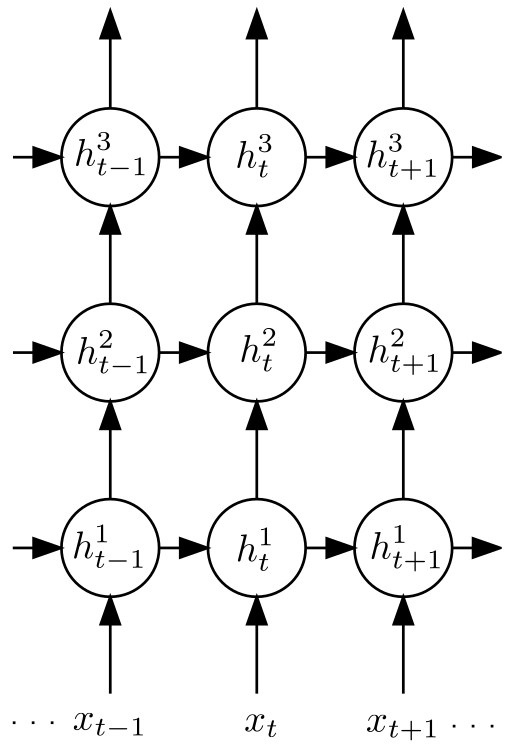
\includegraphics[scale=0.4]{figure/3-layer-lstm}
    \caption[3-layer Recurrent Neural Network]{Computational graph of a 3-layer Recurrent Neural Network~\cite{GravesLSTM}.}
    \label{fig:3-layer-lstm}
\end{figure}

This type of recurrent models were applied in multiple researches~\cite{GravesLSTM}~\cite{SutskeverVL14}~\cite{ZarembaS14}~\cite{treeLSTM}.
Recurrent models with more layers might have the ability to capture longer-term dependency~\cite{treeLSTM}.
In practice, the number of layers \(l\) is treated as hyper-parameter.

\paragraph{Bidirectional Recurrent Neural Networks}\label{sec:bilstm}
In some sequential data prediction problem, an output does not only depends on the input sequence before it but also the input sequence after it.
Additionally, some dependencies are easier to capture when the input is processed in reverse order.
In those cases, Bidirectional Recurrent Neural Networks might have advantages over the basic RNNs~\cite{GravesLSTM}~\cite{Graves-thesis}.

Given an input sequence \(\overrightarrow{I} = \{i_0,\ldots,i_n\}\), we define the reverse input sequence of \(\overrightarrow{I}\) as \(\overleftarrow{I} = \{j_0,\ldots,j_n\}\) with \(j_t = i_{n-t}\).
Using two RNNs \(r_0\) and \(r_1\), the formula of Bidirectional Recurrent Neural Networks can be expressed as follow:
\begin{align}
    \overrightarrow{O} &= r_0(\overrightarrow{I}) &\\
    \overleftarrow{O} &= r_1(\overleftarrow{I}) &
\end{align}
\(\overrightarrow{O}\) and \(\overleftarrow{O}\) can be combined in different ways depend on tasks and settings~\cite{GravesLSTM}~\cite{Graves-thesis}~\cite{treeLSTM}.

\begin{figure}[H]
    \centering
    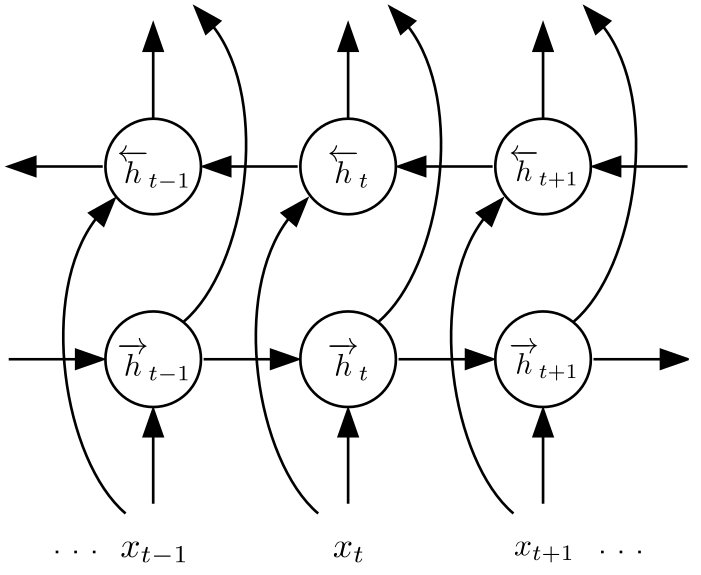
\includegraphics[scale=0.4]{figure/blstm}
    \caption[Bidirectional Recurrent Neural Network]{Computational graph of a Bidirectional Recurrent Neural Network~\cite{GravesLSTM}.}
    \label{fig:blstm}
\end{figure}

\paragraph{Multiple Layers Bidirectional Recurrent Neural Networks}
Given any Recurrent architects \(r\), we can define two operations on it: bidirectional operation \(B(r)\) and multi-layer operation \(M(r, l)\) with \(l\) as the number of layers added.
Using these operators, we can assemble an infinite number of new recurrent architects.
For example the architects illustrated in Fig.\ref{fig:dblstm} can be expressed as \(M(B(lstm), 2)\).

\begin{figure}[H]
    \centering
    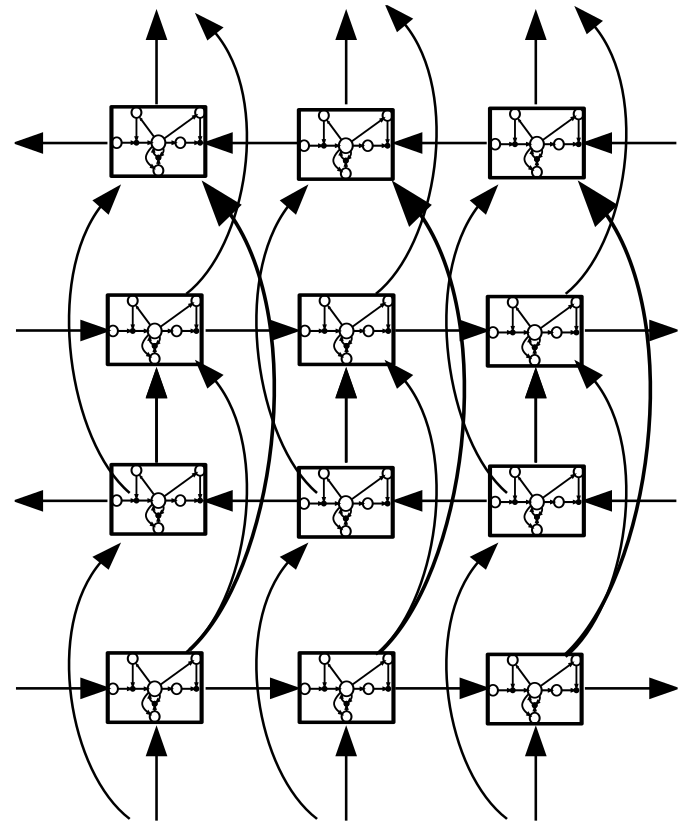
\includegraphics[scale=0.4]{figure/dblstm}
    \caption[Deep Bidirectional Recurrent Neural Network]{Computational graph of a Deep Bidirectional Recurrent Neural Network~\cite{GravesLSTM}.}
    \label{fig:dblstm}
\end{figure}

\subsection{Tree-Structured Long Short-Term Memory Networks (Tree-LSTMs)}\label{sec:treelstm}
Compare to other network architects, Recurrent Neural Networks have a great advantage in handling sequential, arbitrary length input (e.g. sentences, paragraphs, a sequence of frame in a video or a sequence of acoustic unit in a spoken word) but on the other hand, it also comes with the disadvantage of being hard to train~\cite{hardRNN}.
Given a sequence of input, the network has to capture features which can be long-range relationships between inputs~\cite{socher2013recursive}.
One way to improve such structure would be to make these features become easier to capture, in other words, to shorten the length of relationships between inputs.
For the case of sentences, we can present them as syntactic parse trees, in which relevant words and phrases are presented closer to each other in an intuitive way (as human, we understand sentences base on phases and phrases base on words).
In this paper~\cite{treeLSTM}, the authors explored this idea by using tree-structured LSTM to combine sentence presentation from its words.
They archive state-of-the-art performance on two tasks: predicting the semantic relatedness of two sentences (SemEval 2014, Task 1~\cite{SemeEvalTask1}) and sentiment classification (Stanford Sentiment Treebank~\cite{socher2013recursive}).


Given the advantages of tree structure over it sequential counterpart, we will apply this theory to our model in \hyperref[sec:VTtree]{4.1.1} and \hyperref[sec:CNNtree]{4.1.2}.
Their experiments were originally implemented in \hyperref[sec:torch]{Torch7}\footnote{\url{https://github.com/stanfordnlp/treelstm}}, for the purpose of extending their models and doing more experiments, we re-implemented\footnote{\url{https://github.com/ttpro1995/TreeLSTMSentiment}} their models in \hyperref[sec:pytorch]{PyTorch}.

As we only interested in the task of sentiment analysis, the experiment and result related to the task of semantic relatedness will not be presented.

\subsubsection{Method}
\paragraph{Child-Sum Tree-LSTMs}
Given a tree, we denote \(C(j)\) as set of children of node \(j\).
The step of calculation inside Child-Sum Tree-LSTM node \(j\) can be expressed as follow~\cite{treeLSTM}:
\begin{align}
      \tilde{h_j} &= \sum_{k \in C(j)} h_k &\label{eq1:2}\\
      i_j &= \sigma{(W^{(i)}x_j + U^{(i)}\tilde{h_j} + b^{(i)})} &\label{eq1:3}\\
      f_{jk} &= \sigma{(W^{(f)}x_j + U^{(i)}h_k + b^{(f)})}, \qquad  \forall k \in C(j) & \label{eq1:foget1}\\
      o_j &= \sigma{(W^{(o)}x_j + U^{(o)}\tilde{h_j} + b^{(o)})} &\label{eq1:5}\\
      u_j &= \tanh{(W^{(u)}x_j + U^{(u)}\tilde{h_j} + b^{(u)})} &\label{eq1:6}\\
       c_j &= i_j \odot u_j + \sum_{k \in C(j)} f_{jk} \odot c_k & \\
    h_j &= o_j \odot \tanh{(c_j)} &
\end{align}

As Child-Sum Tree-LSTMs has the ability to combine node with an arbitrary number of children, it is can be applied to compose sentence based on it dependency parse tree.
This application was named by the authors as \textbf{Dependency Tree-LSTMs}~\cite{treeLSTM}.

\paragraph{N-ary Tree-LSTMs}
Given a tree, we denote \(C(j)\) as the set of children of node \(j\) and \(N\) as the maximum number of children a node can have.
We will assume that the number of child in a node is always \(0\) or \(N\).
If a node has no children nodes, we call it a leaf-node, else, it will be called a composer-node.

The calculation steps inside leaf-node (leaf-module) \(j\) can be expressed as follow:
\begin{align}
    o_j &= \sigma{\left( W^{(o)} x_j + a^{\left(o\right)}\right)} & \\
       c_j &= W^{(c)} x_j + a^{(c)} & \\
    h_j &= o_j \odot \tanh{\left(c_j\right)} &
\end{align}

The calculation steps inside composer-node (composer-module) \(j\) can be expressed as follow:
\begin{align}
      i_j &= \sigma{ \left(\sum_{l=1}^{N}U_l^{(i)} h_{jl} + b^{(i)} \right) } &\label{eq:9}\\
      f_{jk} &= \sigma{\left(\sum_{l=1}^{N}U_{kl}^{\left(f\right)} h_{jl} + b^{\left(f\right)}\right)}, \qquad  \forall k \in C(j) & \label{eq:foget2}\\
      o_j &= \sigma{\left( \sum_{l=1}^{N}U_l^{\left(o\right)} h_{jl} + b^{\left(o\right)}\right)} &\label{eq:11}\\
      u_j &= \tanh{\left( \sum_{l=1}^{N}U_l^{\left(u\right)} h_{jl} + b^{\left(u\right)}\right)} &\label{eq:12}\\
       c_j &= i_j \odot u_j + \sum_{k \in C\left(j\right)} f_{jk} \odot c_{jl} & \\
    h_j &= o_j \odot \tanh{\left(c_j\right)} & \\
\end{align}

Different from Child-Sum Tree-LSTMs forget gate in Eq.\eqref{eq1:foget1}, N-ary Tree-LSTMs chooses what to forget based on all it children as in Eq.\eqref{eq:foget2}.
Also, each the combination of \(h_{jl}\) in Eqs.\eqref{eq:9},\eqref{eq:11}, \eqref{eq:12} are parameterize by \(U_l^{(i)}\), \(U_l^{(o)}\) and \(U_l^{(u)}\) respectively, compares to linear transformation of sum (Eqs.\eqref{eq1:2}, \eqref{eq1:3}, \eqref{eq1:5}, \eqref{eq1:6}) in Child-Sum Tree-LSTMs.

Knowing that any constituency parse tree can always be presented in a binarized form, to compose a sentence the authors applied 2-ary Tree-LSTMs on the binarized constituency parse tree of that sentence.
This combination was named by the authors as \textbf{Constituency Tree-LSTMs}~\cite{treeLSTM}.

\paragraph{Output module} Denoting sequence of words spanned by a sub-tree rooted at node \(j\) as \(\{x\}_j\).
For both Dependency Tree-LSTMs and Constituency Tree-LSTMs when applying on the task of sentiment analysis, the prediction at node \(j\) can be computed by an output-module as follow~\cite{treeLSTM}:

\begin{align}
      \hat{p_{\theta}}(y \mid \{x\}_j ) &= softmax( W^{(s)} h_j + b^{(s)}) & \\
      \hat{y_j} &= \underset{y}{\mathrm{argmax}} \; \hat{p_{\theta}}(y \mid \{x\}_j ) &
\end{align}

The authors use negative log-likelihood with \(L2\) regularization as loss function~\cite{treeLSTM}.

\paragraph{Training technique and hyper-parameters}
Glove vectors~\cite{glove} was used to initialize word-embedding.
The words presentation were updated with learning rate 0.1 while other parameters in the network were update using AdaGrad~\cite{adagrad} with learning rate 0.05.
Batch-size was set to 25.
\(L2\) regularization was applied at each mini-batch with weight of \(10^{-4}\).
The authors also added a dropout layer~\cite{dropout} with dropout rate of \(0.5\) before each output-module.

\subsubsection{Results and Discussion}
\begin{table}[H]
\centering
\begin{tabular}{l c}
 \hline
 \hline
 Method & Accuracy \\ [0.5ex]
 \hline
 \hline
 \\
 RAE~\cite{socher2013recursive} & 82.4 \\
 MV-RNN~\cite{socher2013recursive} & 82.9 \\
 RNTN~\cite{socher2013recursive} & 85.4 \\
 DCNN~\cite{DCNN} & 86.8 \\
 Paragraph-Vec~\cite{ParagraphVec} & 87.8 \\
 CNN-non-static~\cite{KimCNN} & 87.2 \\
 CNN-multichannel~\cite{KimCNN} & 88.1 \\
 DRNN~\cite{IrsoyDRNN} & 86.6 \\ [0.5ex]
 \hline
 \\
 LSTM~\cite{originLSTM} & 84.9 (0.6) \\
 Bidirectional LSTM~\cite{GravesLSTM} & 87.5 (0.5) \\
 2-layer LSTM~\cite{GravesLSTM} & 86.3 (0.6) \\
 2-layer Bidirectional LSTM~\cite{GravesLSTM} & 87.2 (1.0) \\ [0.5ex]
 \hline
 \\
 Dependency Tree-LSTM~\cite{treeLSTM} & 84.9 (0.6) \\
 Constituency Tree-LSTM~\cite{treeLSTM} &  \\
 \; with randomly initialized vectors & 82.0 (0.5) \\
 \; Glove vectors, fixed & 87.5 (0.8) \\
 \; Glove vectors, tuned & 88.0 (0.3) \\
 \hline
 \hline
\end{tabular}
\caption[Tree-LSTM test result]{Test set accuracies on Stanford Sentiment Treebank with binary setting.
In the first block, the results were reported in their original papers.
The second block contains results produced by sequential models and tree-structured models for the third block.
For each models in the second and third block, mean accuracy over 5 runs (standard deviation in parentheses) was reported}
\label{table:1}
\end{table}

The results presented in Table\ref{table:1} support the hypothesis that tree-structured LSTMs are better than sequential LSTMs when applying on sequences which have nested grammar~\cite{treeVSseq}.
We should notice that good word embedding give a great boost to the system~\cite{Luong_betterword}, fine-tune also beneficial.

\begin{figure}[H]
    \centering
    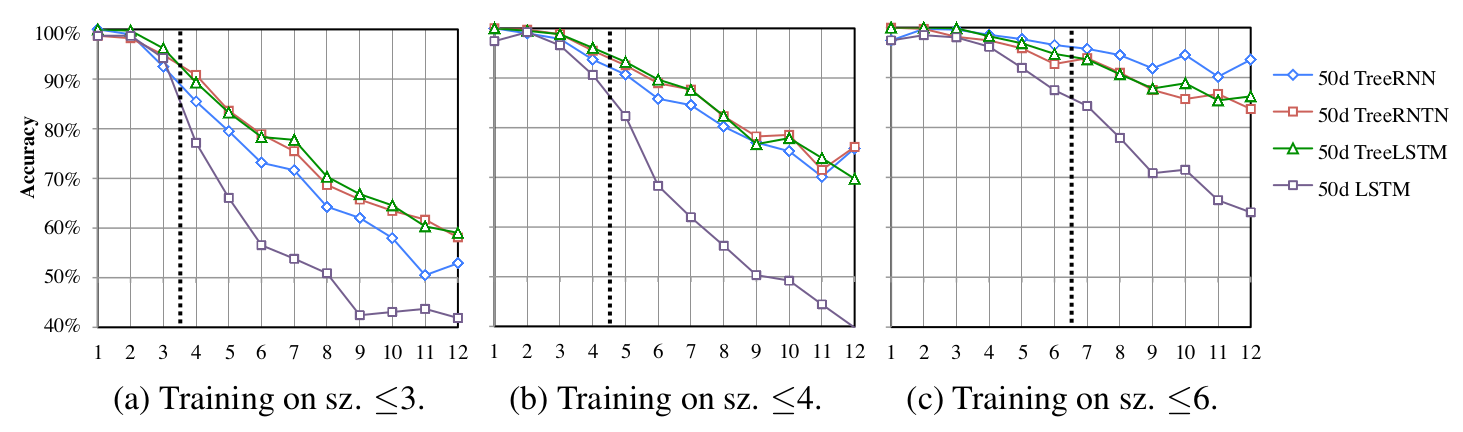
\includegraphics[scale=0.38]{figure/tree-vs-seq}
    \caption[Test accuracy vs sentence length]{Test accuracy on three experiments with increasing limited length of sentences in training data.
The vertical axis is accuracy and the horizontal axis is limited length of sentences in testing data.
Experiments were done with~\cite{socher2013recursive}, TreeRNTN~\cite{socher2013recursive}, TreeLSTM~\cite{treeLSTM} and LSTM~\cite{originLSTM}.
50 is the number of dimension of hidden stat \(h\).
This data set was generated using an artificial recursively defined language~\cite{bowman-treevslstm}.}
    \label{fig:tree-vs-seq}
\end{figure}
\label{sec:tree-discuss}
\textbf{Advantages of Tree-LSTMs} are presented in several studies~\cite{need-tree}~\cite{bowman-treevslstm}: \label{treelstm-advantage}
\begin{itemize}
\item In case the input sequence is belong to recursively defined language, given only a small subset of the data with limited length sentences, tree structures model have better ability to generalize compare to sequential ones.
But when we increase the limited length sentences, the advantage of tree over sequential models decrease fast~\cite{bowman-treevslstm}.
This can be demonstrated in Fig.\ref{fig:tree-vs-seq}.
\item Tree can breaks down complicated sentences into simpler phrases, which make it easier for generalization~\cite{knowledge-matter}~\cite{need-tree}.
\item Some features which are far apart when a sentence is presented as sequence become closer when it is presented as tree~\cite{need-tree}.
\end{itemize}


\textbf{Disadvantages of Tree-LSTMs} including:\label{treelstm-drawback}
\begin{itemize}
\item Sentences can be wrongly parsed, especially when comments are expressed in informal language.
The performance of the system depends on the parser being used.
\item When combining a sub-tree, that sub-tree has no information about its context.
Compared to sequential structures, when combining an input (e.g. word, phrase), the network already has the left context information of that input~\cite{shift-reduce}.
\item A closer look at Eqs.\eqref{eq1:6},\eqref{eq:12} reveal that, Tree-LSTMs have only a logistic regression at each node to capture features.
We think this is the reason why Kim's CNN\ref{kim-cnn} can outperform TreeLSTMs.
\item Tree-LSTMs can not be trained using batch in parallelism. But this disadvantage can be overcome thank to Tree-LSTMs shift-reduce implementation~\cite{shift-reduce}.
\end{itemize}


\subsection{Convolutional Neural Networks (CNNs)}\label{kim-cnn}
In Table\ref{table:1}, we can see that the best model is not Constituency Tree-LSTM but CNN-multichannel~\cite{KimCNN}, which was originally presented in this paper.
With only a one-layer \hyperref[sec:cnn]{Convolution Neural Network}, and general hyper-parameter tuning, the author was able to archive state-of-art\footnote{in 2014} performance on several NLP tasks, which include sentiment analysis (\hyperref[sec:sst]{Stanford Sentiment Treebank}~\cite{socher2013recursive}).
The paper also successfully adapted the idea of training CNN on multiple channels image in Computer Vision to training CNN on multi-channel words embedding for sentence\footnote{Implementation of this paper can be found at \url{https://github.com/yoonkim/CNN\_sentence}}.

\begin{figure}[H]
    \centering
    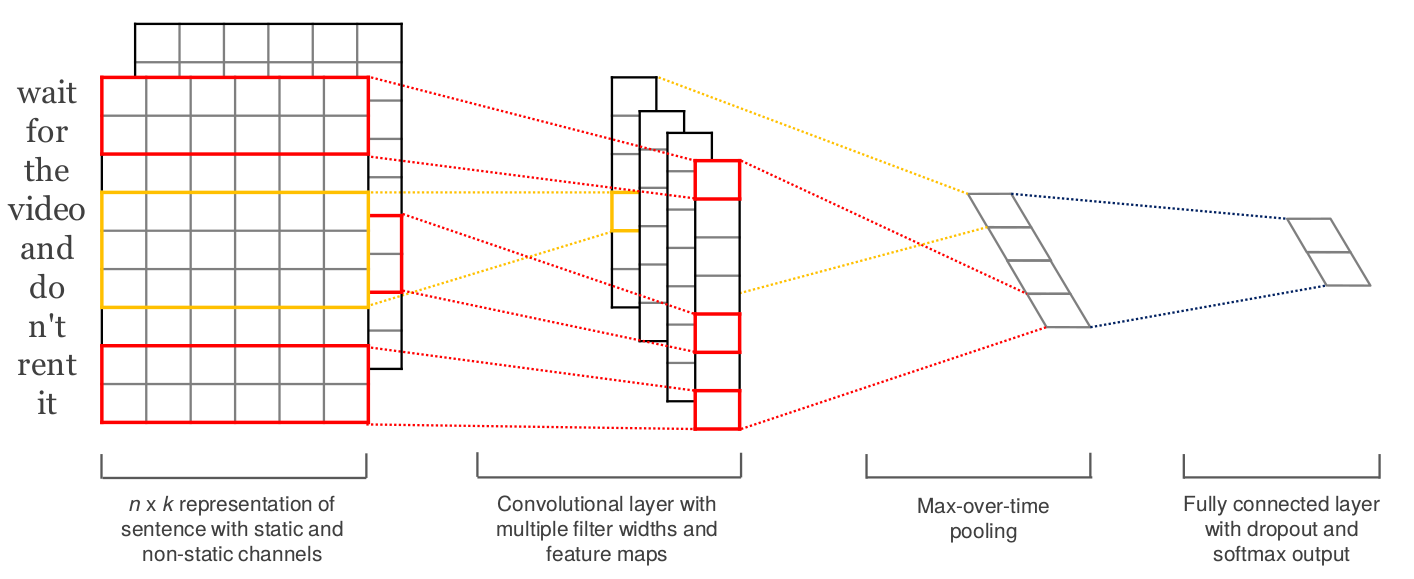
\includegraphics[scale=0.33]{figure/sentencecnn}
    \caption[CNN with two embedding channel]{Structure of CNN with two word embedding channels of the same sentence}
    \label{fig:multi-cnn}
\end{figure}

\subsubsection{Method}
Let denote \(\bm{x_i \in \mathbb{R}^d}\) as a \(d\)-dimension vector presentation of word-\(i\)th in a sentence.
Given a sentence \(\bm{s}\) of length \(n\), we can present a sub-sequence of words in the sentence which start at word-\(i\)th and end at word-\(j\)th as:
\begin{align}
    x_{i:j} &= x_i \oplus x_{i+1} \oplus ... \oplus x_{j} &\label{concat}
\end{align}
In Eq.\eqref{concat}, operator \(\bm{\oplus}\) do concatenation. Therefore, \(x_{i:j} \in \mathbb{R}^{d(j-i+1)}\).

\paragraph{Convolution filter} \label{conv-filter} Now we are ready to define a filter.
A filter with window size \(\bm{l}\) is a vector \(\bm{w \in \mathbb{R}^{ld}}\) which applies on vector presentations of word-\(i\)th to word-\((i+l-1)\)th through the following equation:
\begin{align}
    c_i &= f(w \cdot x_{i:i+l-1} + b) &\label{filter}
\end{align}

In Eq.\eqref{filter}, \(\bm{b \in \mathbb{R}}\) as bias term and \(\bm{f}\) is a activation function.

\begin{figure}[H]
    \centering
    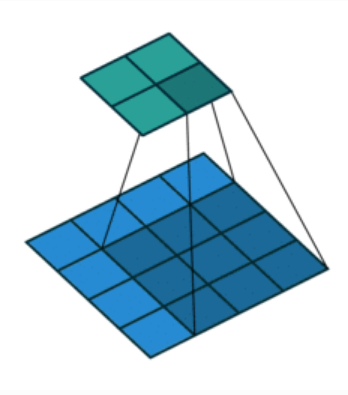
\includegraphics[scale=0.4]{figure/no_padding}
    \caption[Convolution filter policy]{No padding and unit strides policy when applying a filter on a matrix.}
    \label{fig:no_padding}
\end{figure}

By slicing the filter through the sentence we can get vector \(\bm{c}\) which can be view as a feature map of sentence \(s\).
In this paper, the author use no padding and unit strides policy (Fig.\ref{fig:no_padding}), which gives \(c \in \mathbb{R}^{n-l+1}\).

\paragraph{Max-over-time pooling}\label{sec:max-overtime-pooling} Given the feature map, the author then take the maximum value in it \(\bm{c^* = max\{c\}}\) (max-over-time pooling~\cite{nlp-scratch}), which is a sentence feature produced by the filter.
So, convoluting a filter with the sentence will produce one feature \(\bm{c^* \in \mathbb{R}}\).

\paragraph{Sentence presentation} Applying \(\bm{k}\) filters on the sentence, and we will have a feature vector \(\bm{p \in \mathbb{R}^k}\).
In case of sentiment classification, the feature vector \(p\) can be fed to a classifier like the one in the last layer of the architect presented in Fig.\ref{fig:multi-cnn}.

\paragraph{Multi-channel input} Given that the sentence is presented by a set of channels \(\bm{Z}\) and the network has \(\bm{k}\) filters.
We will modify Eq.\eqref{filter} as follow:

\begin{align}
    \forall h \in Z, \; \; \hat{c}_{ih} &= f(w \cdot x_{i:i+l-1} + b)& \\
    c_i &= \sum_{h \in Z} \hat{c}_{ih}&
\end{align}

The rest of the system is unchanged compared to a single-channel one.
The whole process is illustrated in the first two layers of the architect in Fig.\ref{fig:multi-cnn}.

\paragraph{Experimented models} The author did experiments with several variations:

\begin{itemize}
      \item \textbf{CNN-rand:} One channel word embedding are randomly initialized and updated during the training process.\label{cnn-rand}
    \item \textbf{CNN-static:} One channel word embedding are initialized with word2vec~\cite{word2vec} and not updated during the training process even for unknown randomly initialized new word.\label{cnn-static}
    \item \textbf{CNN-non-static:} One channel word embedding are initialized with word2vec and updated during the training process.\label{cnn-non-static}
    \item \textbf{CNN-multichannel:} Two channels word embedding are initialized with word2vec. One of the channel is updated during the training process and the other is kept static.\label{cnn-multichannel}
\end{itemize}
\paragraph{Training method and hyper-parameters}
Rectifier~\cite{rectifier} were use as activation function.
The author used window size 3, 4 and 5, each of which have 100 filters, the max-over-time pooling layer will produce a 300-dimension sentence presentation vector.
Dropout layer was used after the max-over-time pooling layer with dropout-rate of \(0.5\).
Batch-size was set to 50.
All weight vectors were normalized to have \(\norm{w}_2 = 3\) whenever \(\norm{w}_2 > 3\).
Adadelta~\cite{adadelta} was used as optimizer of the networks.
When training on Stanford Sentiment Treebank, each labeled sub-tree's span was treated as an example.
At test phase, each input is a sentence, and output is a sentiment prediction for that sentence.

\subsubsection{Results and Discussion}\label{kimcnn-drawback}
\begin{table}[H]
\centering
\begin{tabular}{l c}
 \hline
 \hline
 Method & Accuracy \\ [0.5ex]
 \hline
 \hline
 \\
 CNN-rand & 82.7 \\
 CNN-static & 86.8 \\
 CNN-non-static & 87.2 \\
 CNN-multichannel & 88.1 \\
 \hline
 \hline
\end{tabular}
\caption[CNN test result]{Test set accuracies on Stanford Sentiment Treebank with binary setting. These models are presented in Sec.\ref{cnn-multichannel}.
A comparison with models from different works has been presented in Sec.\ref{table:1}}
\label{table:KimCNN}
\end{table}

Multiple channels with one static and one for fine-tuning help the network to better generalize.
There is a drawback in CNN-multichannel: although max-over-time pooling largely simplified the network (which is good for preventing over-fit), it only tell if a feature appears in a sentence or not, the information about position of the feature is ignored.\label{kim-drawback}
The next research in Sec.\ref{cnn-rnn}  improve CNN-multichannel based on this drawback.


\subsection{Combining Convolutional and Recurrent Neural Network (CNN-RNN)}\label{cnn-rnn}
As we have observed the drawback of max-over-time pooling layer in Sec.\ref{kimcnn-drawback}, we will analyze how the authors of this paper~\cite{cnn-rnn} tackled it.

\subsubsection{Method}
\begin{figure}[H]
    \centering
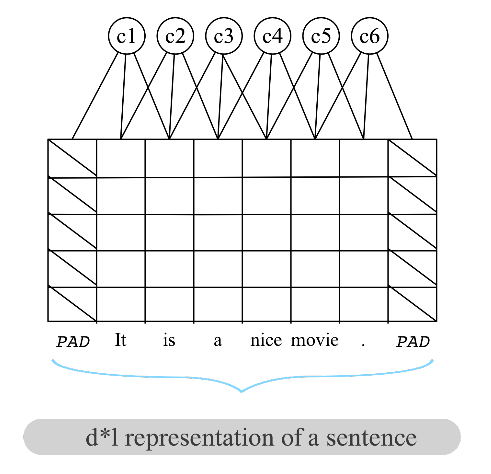
\includegraphics[scale=0.45]{figure/conv-word}
    \caption[Convolution with padding]{A convoluting filter slicing through a sentence.
    Padding was added.}
    \label{fig:conv-word}
\end{figure}

\paragraph{Preprocessing Sentence} We re-use the definition of convolution filter described in Sec.\ref{conv-filter}.
Given a sentence \(s\), the authors first padding it with \((l-1)\) "dummy-words" on each end of the sentence, with \(l\) as the largest window size among all filters.
After that, the padded-sentence is padded on its right until reaching the length of the longest padded sentence in the data set.
In other words, given that \(m\) is length of the longest sentence in SST, the input of a filter with window size \(l\) will always be a padded-sentence of length \((m + 2(l-1))\).
A filter of size \(k\) then slices through a padded-sentence with unit strides and produces a feature map \(c \in \ \mathbb{R}^{m + 2l - k - 1}\).
This process in illustrated in Fig.\ref{fig:conv-word}

\begin{figure}[H]
    \centering    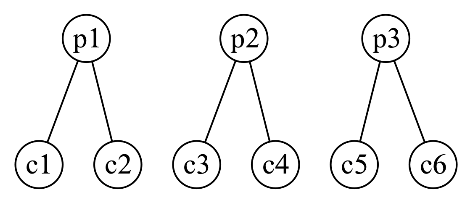
\includegraphics[scale=0.34]{figure/2-max}
    \caption[Max pooling policy]{Max pooling with window size 2 and strides 2 slicing through a feature map}
    \label{fig:2-max-pooling}
\end{figure}

\paragraph{Max pooling layer} A max pooling layer of window size 2, with strides 2, slice through each feature map, and reduce its size by a half.
We will denote this vector \(p \in \mathbb{R}^{\floor{\frac{m + 2l - k - 1}{2}}} \).
This process is illustrated in Fig.\ref{fig:2-max-pooling}


\begin{figure}[H]
    \raggedleft    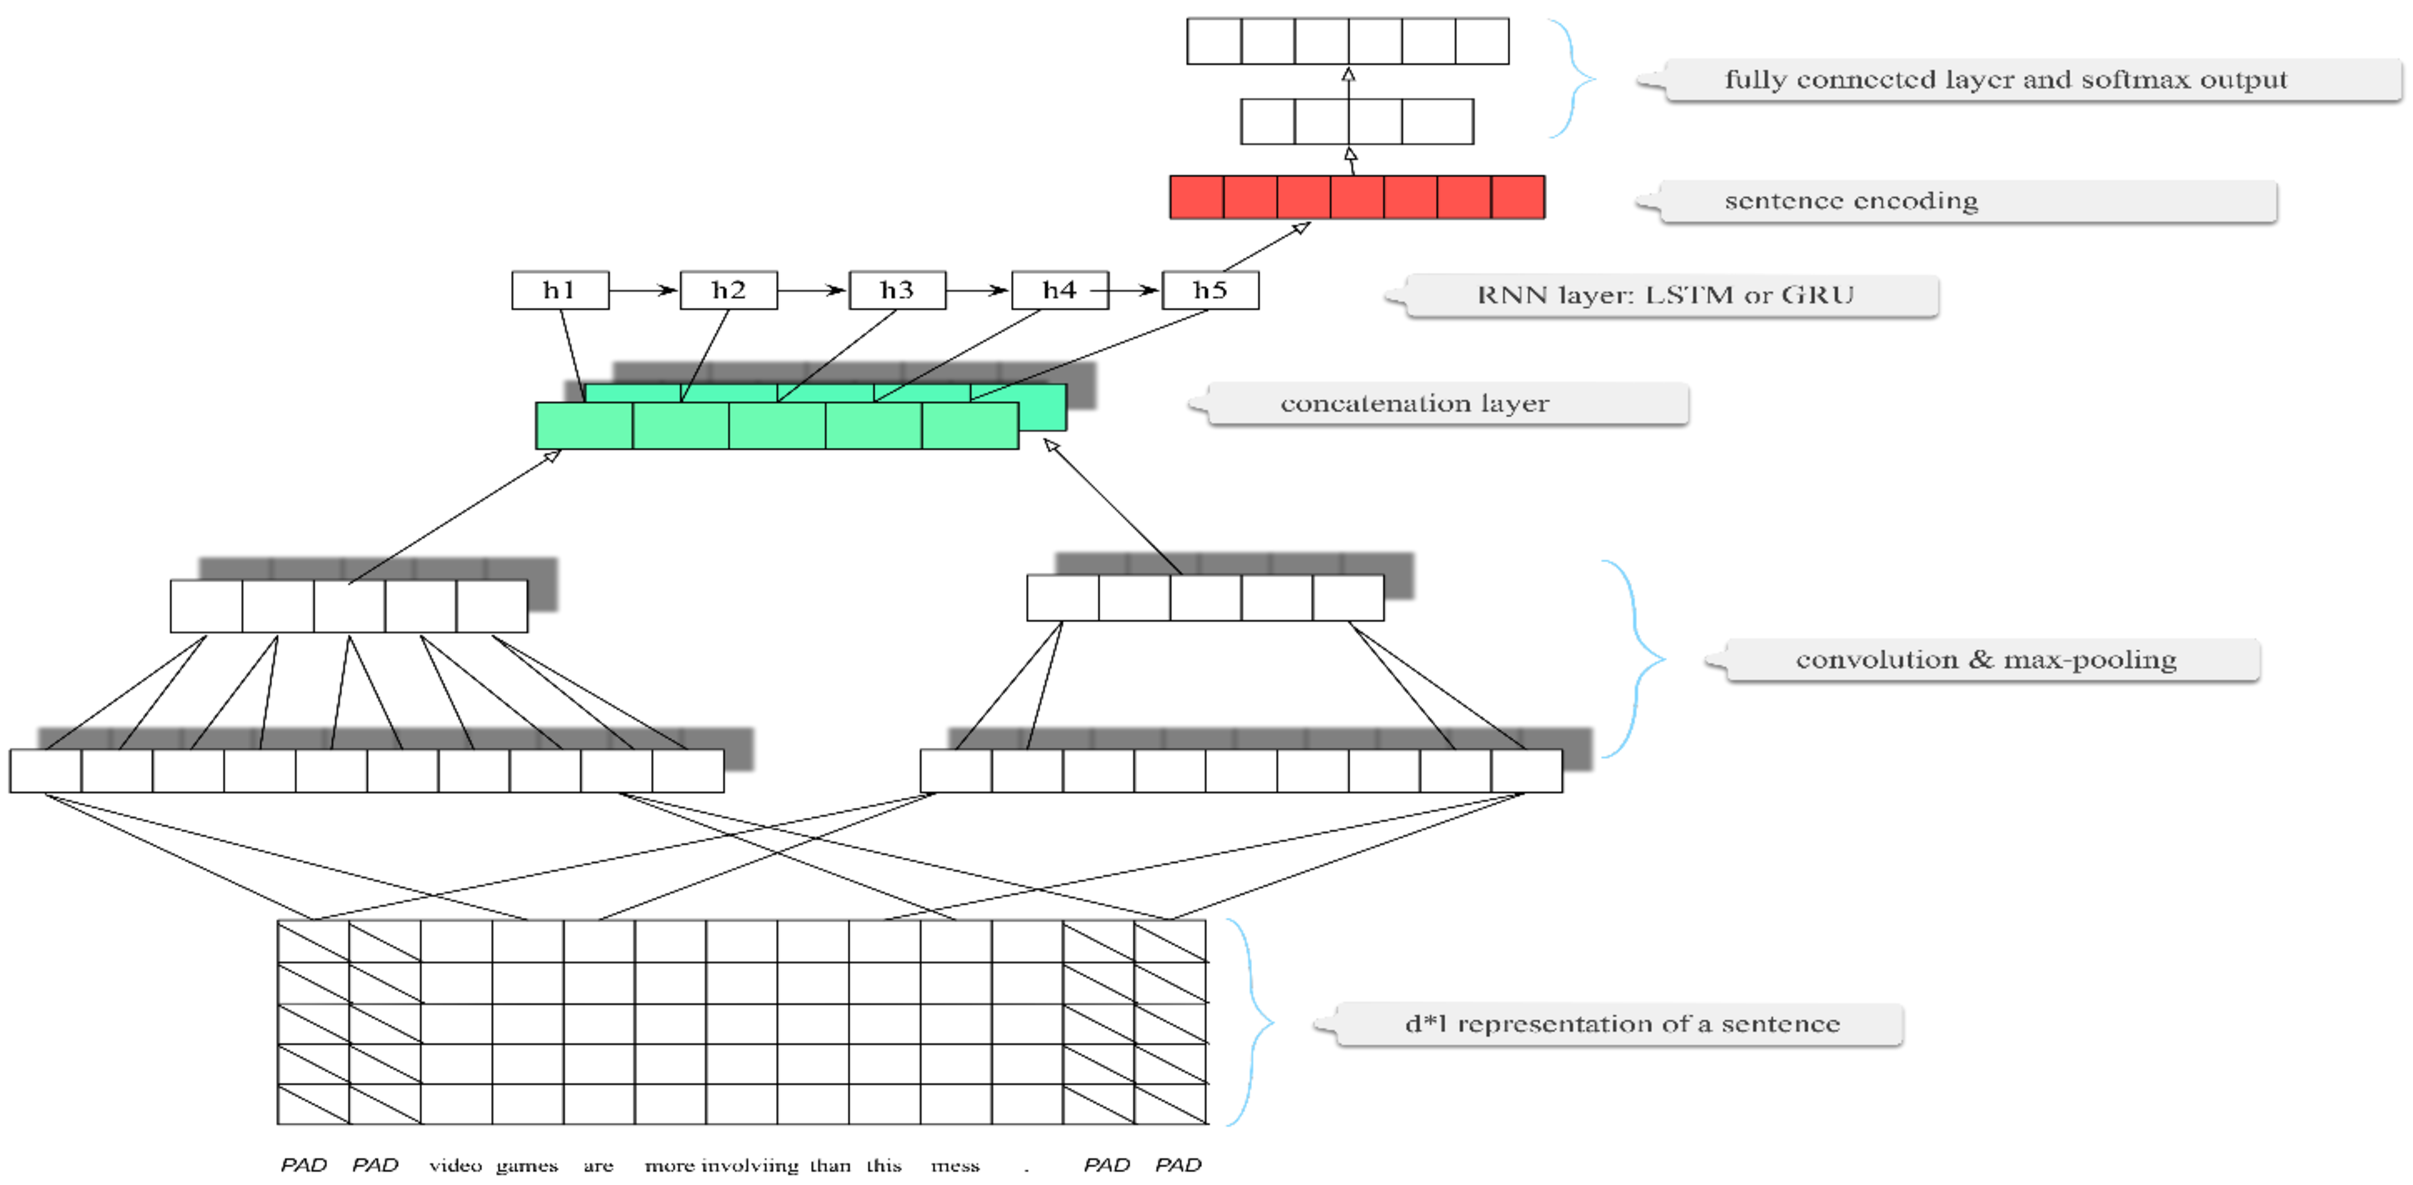
\includegraphics[scale=0.425]{figure/cnn-rnn}
    \caption{CNN-RNN}
    \label{fig:cnn-rnn}
\end{figure}

Note that for filters with different window sizes, the size of feature vectors \(p\) are also different.
This will be problem if we want to compile feature vectors with different size.
To solve this problem, the authors chose only two types of window size: \(4\) and \(5\).
Which results in all feature vectors having the same size.

Given \(n\) filters, the authors then concatenated all the feature vectors into one matrix \(P \in \mathbb{R}^{n \times \floor{\frac{m + 2l - k - 1}{2}}}\), which each row is a feature vectors.
After that, each column in \(P\) treated as an input \(i \in \mathbb{R}^{n}\) for a recurrent neural network, which can be RNN, LSTM or GRU.
The last output of the recurrent neural network can be then fed to MLP for classification.
The whole process is demonstrated in Fig.\ref{fig:cnn-rnn}.

\paragraph{Training method and hyper-parameters}
Word presentation vectors were initialized with word2vec~\cite{word2vec}.
The author used window size 4 and 5, each of which has 200 filters.
When training on Stanford Sentiment Treebank, each labeled sub-tree's span was treated as an example.
At test phase, each input is a sentence, and output is a sentiment prediction for that sentence.
Other hyper-parameters were not specified in this paper, but can be found in the authors' implementation\footnote{\url{https://github.com/ultimate010/crnn}}.

\subsubsection{Results and Discussion}
\begin{table}[H]
\centering
\begin{tabular}{l c}
 \hline
 \hline
 Method & Accuracy \\ [0.5ex]
 \hline
 \hline
 \\
 MAX-GRU & 89.95 \\
 MAX-LSTM & 89.56 \\
 AVG-GRU & 89.61 \\
 \hline
 \hline
\end{tabular}
\caption[CNN-RNN test result]{Test set accuracies on Stanford Sentiment Treebank with binary setting.
The models' names have the following format: \{type pooling layer\}-\{type of RNN\}.
A comparison with models from different works has been presented in Sec.\ref{table:1}}
\label{table:cnn-rnn}
\end{table}

This paper proved that the ability to combine feature based on their position is important for sentence-level sentiment analysis.
This is one way to overcome the disadvantage in Yoon Kim's models (Sec.\ref{kim-drawback}).


\section{Unsupervised pre-training methods}\label{sec:unsupervised-pretrain}
A large number of studies have prove that unsupervised pretraining model can help it greatly generalize~\cite{why-unsupervised}~\cite{greedy-layer}~\cite{greedy-layer-bengio}~\cite{pretrain-1}.
In case of Sentiment Analysis and specifically the task on Stanford Sentiment Treebank, we can identify several challenges that can be overcome using unsupervised pre-train technique~\cite{why-unsupervised}:
\begin{itemize}
\item Given the training data set of SST, the networks have no knowledge about film industry (e.g. movie genres, director, actor, art style).
\item It also does not know human emotions or meaning of their expressions.
\item The networks also have little knowledge about the meaning of phrases, idioms, and even meaning of words based on its' context.
\item The networks might have too many tuning parameters compare to the number of training examples in SST.
Which can lead to over-fitting.
\end{itemize}
We will present several potential methods that are applicable for our models.

\subsection{Natural Language Modeling}\label{sec:nlm}
The goal of language modeling is to model the probability distribution of a word conditioning on the words before it.
More concretely, given a sequence of words (or history) \((w_0, w_1,\ldots,w_n)\), the task of a language model \(M\) is to model the probability distribution \(P_M(w_{n+1}|w_0, w_1,\ldots,w_n)\).
For this task, we can use any model (e.g. recurrent neural network, convolution neural network, MLP) that has the ability to encode an arbitrary sequence of words/symbols (belong to our language).
The encoded context is then used to predict the next word \(w_{n+1}\).
With consideration, the whole system can be trained end-to-end.\footnote{Pytorch implementation: \url{https://github.com/pytorch/examples/tree/master/word\_language\_model}}

We can evaluate a language model by measuring its perplexity on a test data set. Given test data \(T = (w_0, w_1,\ldots,w_n)\), the perplexity \(PP_T\) of a model \(M\) on \(T\) can be calculated as follow~\cite{perplexity}:
\begin{align}
    PP_T(M) &= \frac{1}{\sqrt[n]{\prod_{i=0}^{n} P_M(w_{i}|w_0, w_1,\ldots,w_{i-1})}}&
\end{align}

\label{lm-hypothesis}
\textbf{The advantages} of this approach including:
\begin{itemize}
\item Can be trained on a large number of data sets, with the only condition is that the data sets belong to the language.
\label{unproved:unsupervised-good}
\item If we pre-train our models on Amazon Reviews data set, the models can learn to capture sentiment features, as it needs to predict the distribution of words in comments.
It could also learn more interesting features, such as:
The reviewer cries when watching a good romantic movie, or the viewer praises the novel and then criticizes the movie based on the novel, or how sentiments are being expressed by sentence structures.
This technique has been reported to improve accuracy on Rotten Tomatoes sentiment classification task~\cite{Rotten-Tomato} (which is a super set of Stanford Sentiment Treebank data set (Sec.\ref{sec:sst})).
\end{itemize}

One clear disadvantage of this approach is that we can not use it to unsupervised pre-train tree structured networks.
As tree need full sentence with or full phrase, it can not process arbitrary words sequence.

\subsection{Sentence Encoding}
In this approach, the whole sentence is encoded using some models that we wish to pre-train.
The encoded sentence is then used to predict the words it contains.
The prediction task can be defined in different ways:
\begin{itemize}
\item We can use a small context window around the guesting word.
The words in context window and vector presentation of the sentence can be concatenated/averaged and feed to a classifier as in Fig.\ref{fig:para-vec-1}.

\begin{figure}[H]
    \centering    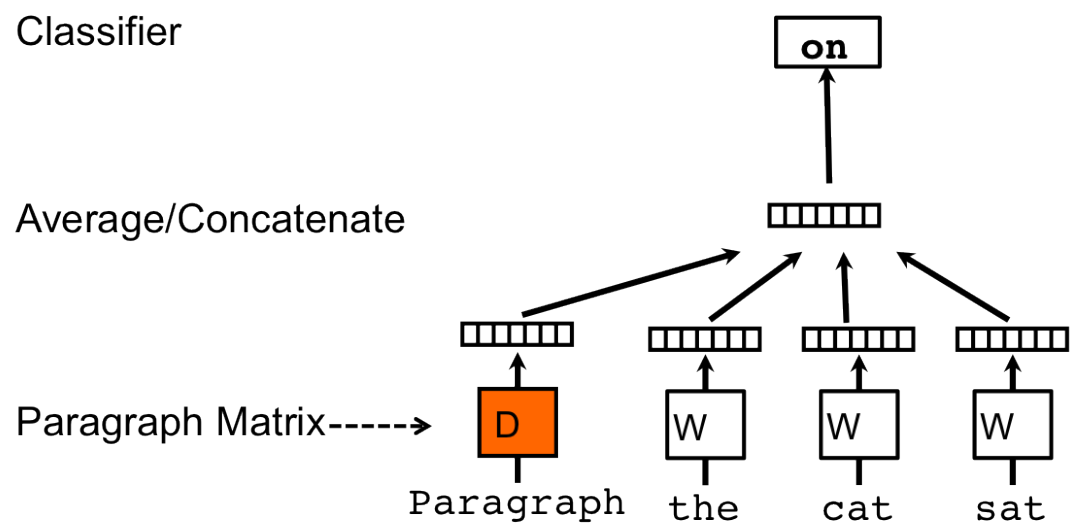
\includegraphics[scale=0.3]{figure/para-vec-1}
    \caption[Distributed Memory Model of Paragraph Vectors (PV-DM)]{Distributed Memory Model of Paragraph Vectors (PV-DM)~\cite{ParagraphVec}}
    \label{fig:para-vec-1}
\end{figure}

\item Another way would be to just use the sentence presentation vector to guest which word it contains as in Fig.\ref{fig:para-vec-2}.

\begin{figure}[H]
    \centering    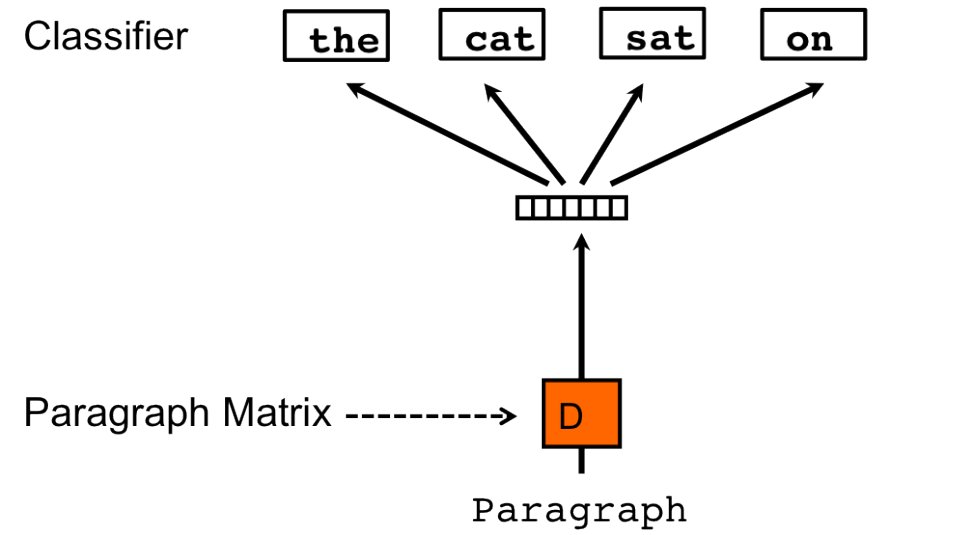
\includegraphics[scale=0.3]{figure/para-vec-2}
    \caption[Distributed Bag of Words version of Paragraph Vector (PV-DBOW)]{Distributed Bag of Words version of Paragraph Vector (PV-DBOW)~\cite{ParagraphVec}}
    \label{fig:para-vec-2}
\end{figure}

\item The third way was inspired by the recent successes of seq2seq learning~\cite{SutskeverVL14}~\cite{semisup-seq2seq}\footnote{A Pytorch implementation of seq2seq models can be found at \url{http://pytorch.org/tutorials/intermediate/seq2seq_translation_tutorial.html}}.
This method use a RNN (e.g. Vanilla RNN, LSTM, GRU in Sec.\ref{sec:RNN}) to encode a sentence then use the same RNN to reconstruct it given its encoded vector~\cite{semisup-seq2seq} as in Fig.\ref{fig:rnn-autoencoder}.
By unsupervised pre-train using this method on Amazon review (Sec.\ref{sec:amazon})), the authors were able to archive dramatic improvement on Rotten Tomatoes sentiment classification task.

\begin{figure}[H]
    \centering    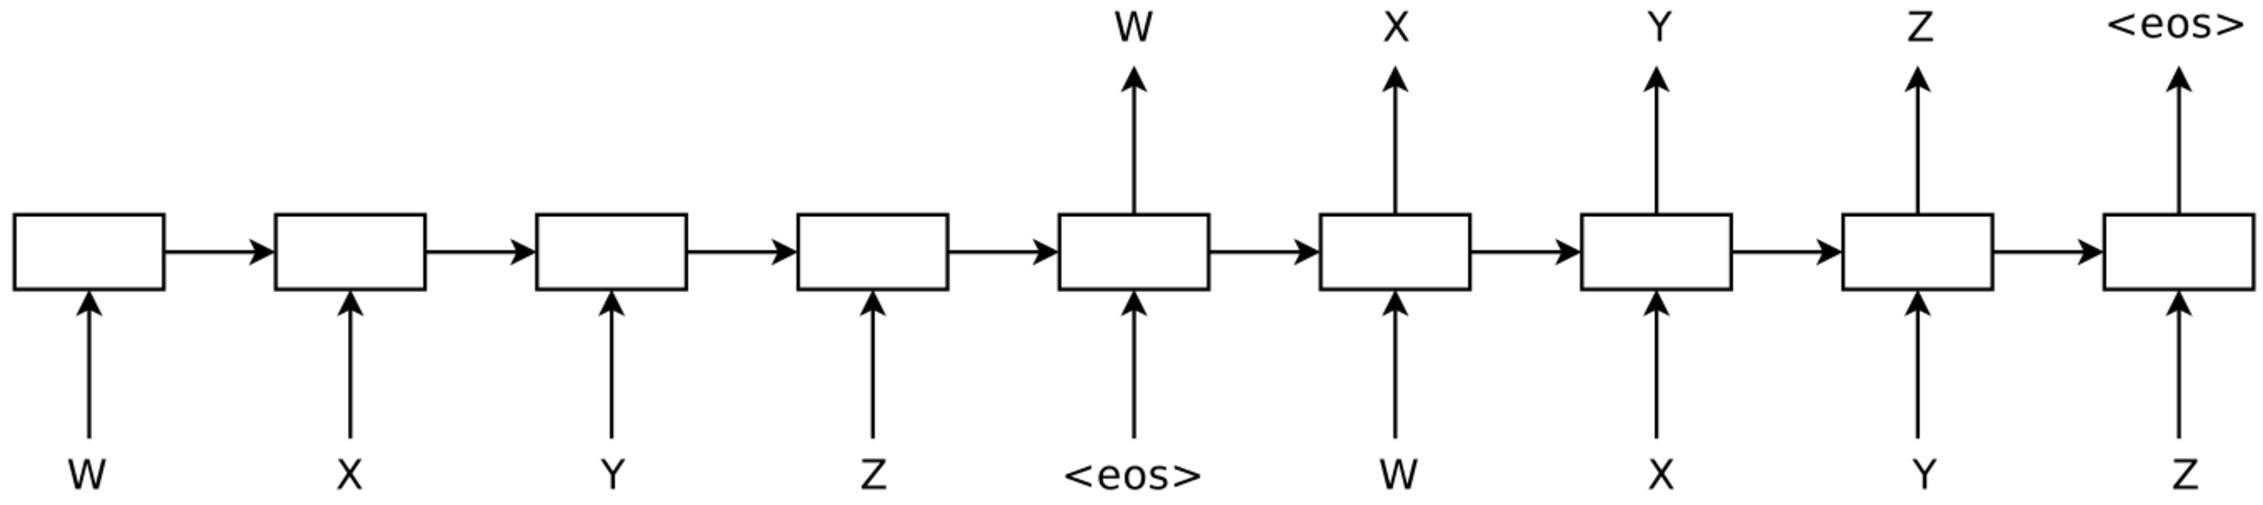
\includegraphics[scale=0.43]{figure/rnn-autoencoder}
    \caption[Sequence Autoencoder]{Sequence Autoencoder processing the sentence "WXYZ"~\cite{semisup-seq2seq}.}
    \label{fig:rnn-autoencoder}
\end{figure}

\end{itemize}

\paragraph{An example of successfully applying unsupervised training technique to improve sentiment analysis on Stanford Sentiment Treebank} \label{sec:2-layer-cnn}
One recent research~\cite{2-layer-cnn} has demonstrated that applying unsupervised training can improve sentiment analysis task on Stanford Sentiment Treebank.

\begin{figure}
    \centering    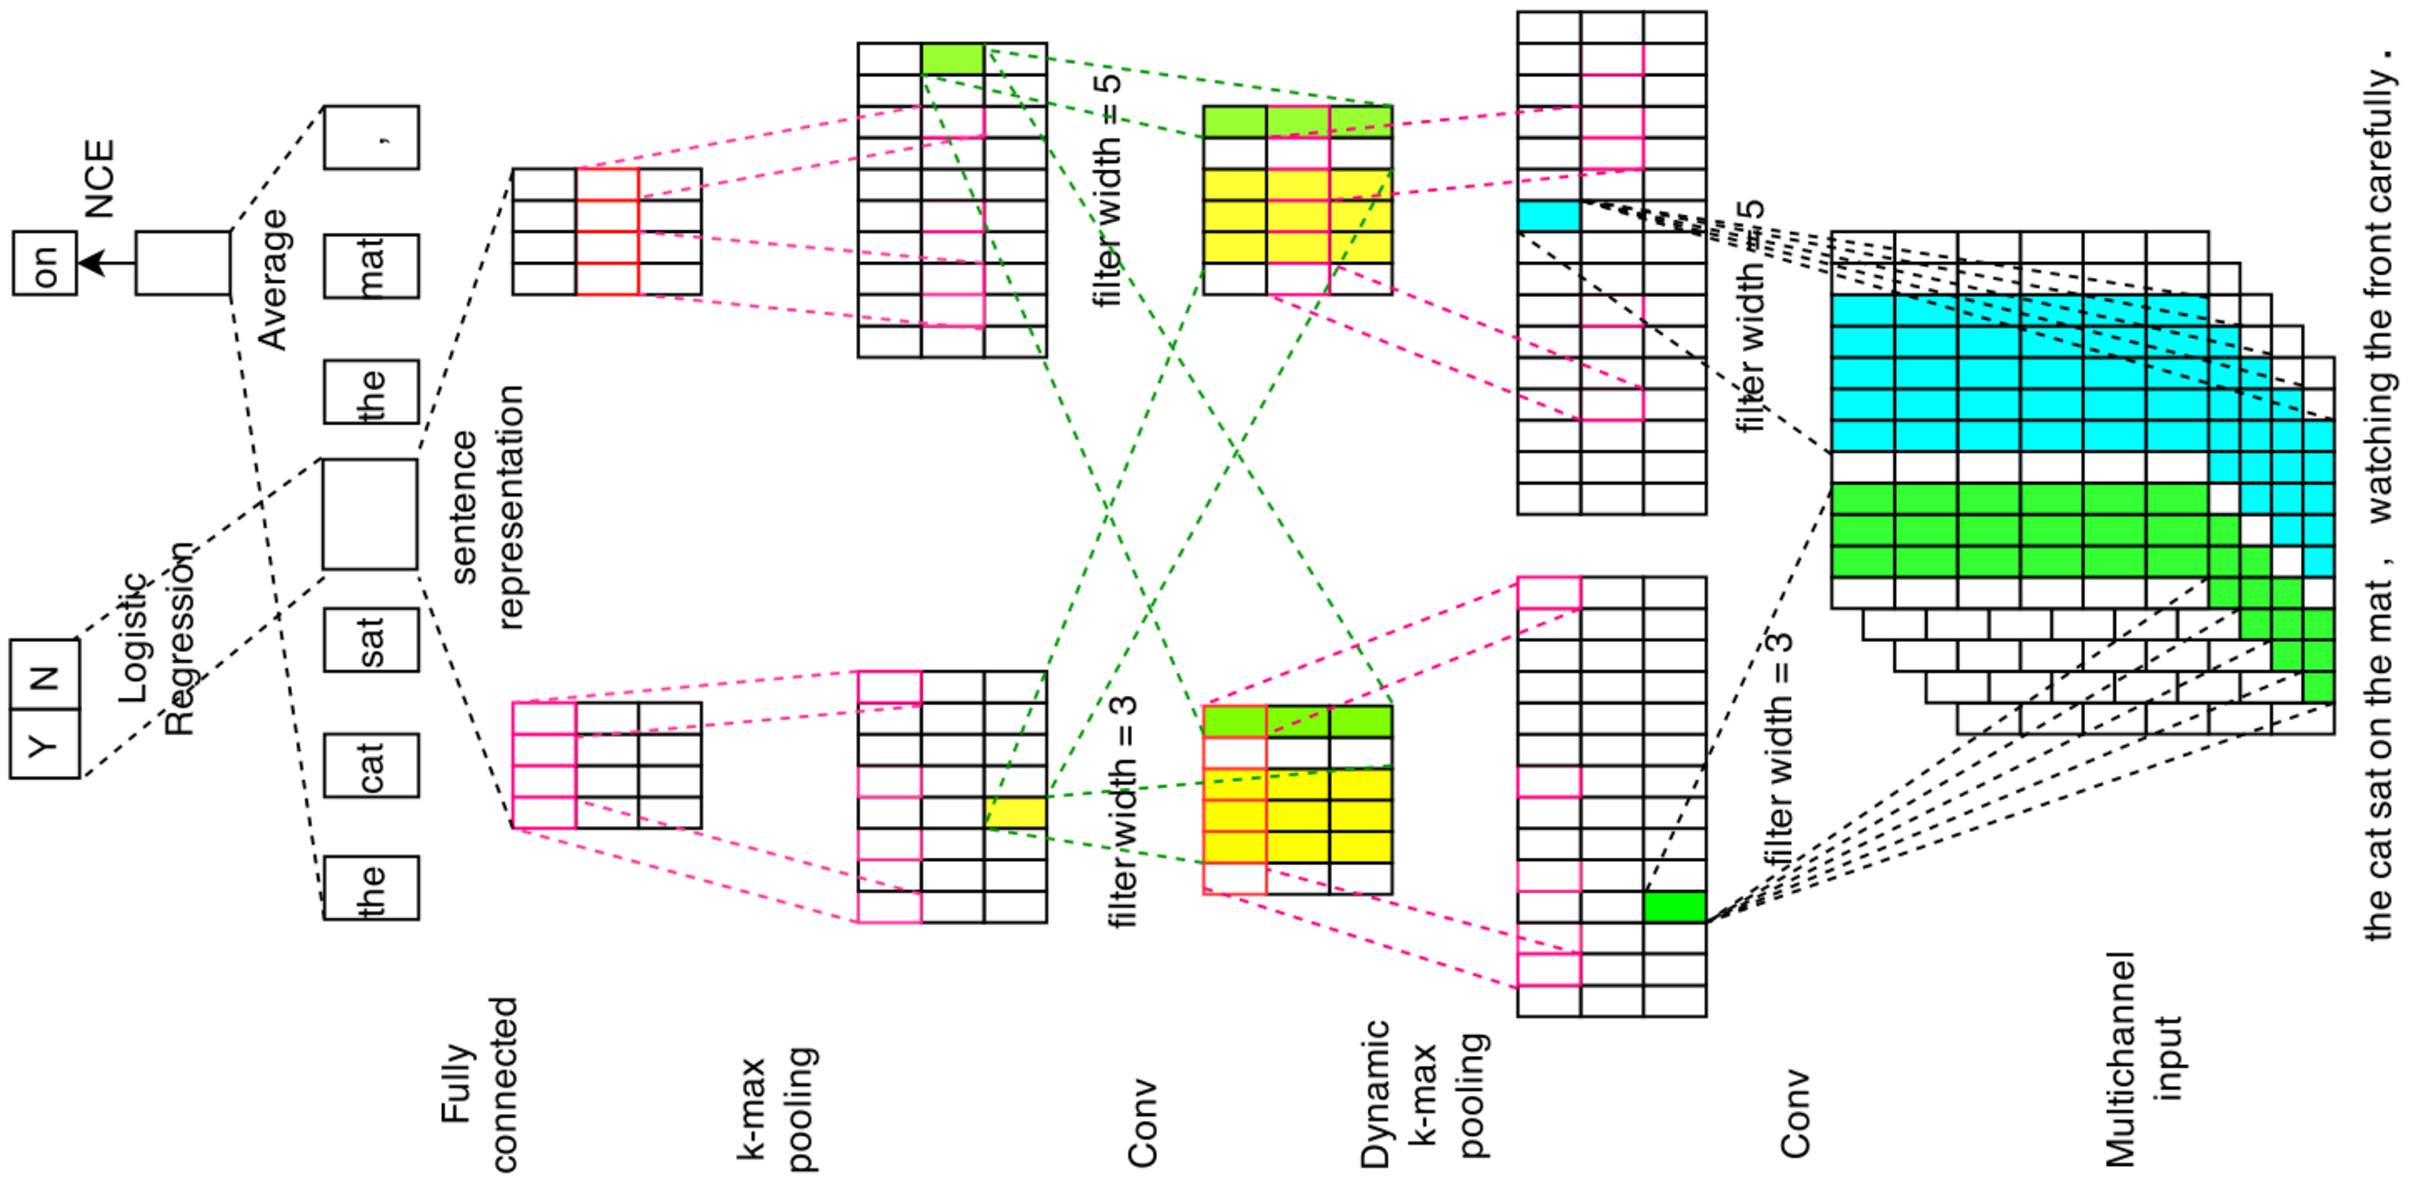
\includegraphics[scale=0.5, angle =-90 ]{figure/2-layer-cnn}
    \caption[2-layer CNN]{Model architect of a multichannel 2-layer CNN during supervised and unsupervised training process~\cite{2-layer-cnn}.}
    \label{fig:2-layer-cnn}
\end{figure}

As illustrated in Fig.\ref{fig:2-layer-cnn}, the first convolution layer and multichannel word embedding of this network are similar to \hyperref[kim-cnn]{Yoon Kim's CNN architect}.
The difference appears after that, instead of using  \hyperref[sec:max-overtime-pooling]{max pooling overtime layer} to produce sentence encoding vector, the authors used Dynamic k-max Pooling~\cite{DCNN} layer with another convolution layer and a k-max pooling layer~\cite{DCNN}.

With large number of parameter, their model prone to over-fitting, to tackle this problem, the authors unsupervised pre-train their model on large unlabeled data set using setting similar to Distributed Memory Model of Paragraph Vectors (PV-DM)~\cite{ParagraphVec} (Fig.\ref{fig:para-vec-1}).
Given a model \(M\) which the authors want to pre-train, and a sentence \(s\) in the data set used for pre-training process, the sentence presentation \(p\) is computed as \(M(s)\).
Define the context of the target word \(w_i\) as \(C = \{w_{i-t},\ldots,w_{i-1}, w_{i+1},\ldots,w_{i+t}\}\), the feature vector used to predict word \(w_i\) is computed by averaging word presentation vectors of the words in \(C\) and sentence encoding \(p\)~\cite{2-layer-cnn}.

On overall, their system was able to archive accuracy of \(89.4\%\) on binary setting of sentiment analysis.
With pre-training step removed from the training process, the model only archived accuracy of \(87.6\%\), which proved the significant contribution of pre-training step.~\cite{2-layer-cnn}
